%
% teil3.tex -- Beispiel-File für Teil 3
%
% (c) 2020 Prof Dr Andreas Müller, Hochschule Rapperswil
%
% !TEX root = ../../buch.tex
% !TEX encoding = UTF-8
%
\section{Variationsprinzip bei einem genetischen Algorithmus
\label{buch:paper:varalg:section:genetic_algorithm_process}}
\kopfrechts{Variationsprinzip beim genetischen Algorithmus}
Ein genetischer Algorithmus nutzt nach ChatGPT das Variationsprinzip, 
das wie folgt definiert wird:
\begin{quote}
Das Variationsprinzip ist ein grundlegendes Konzept in der 
evolutionären Computertechnik, insbesondere in genetischen 
\index{evolutionäre Computertechnik}%
Algorithmen. Es besagt, dass genetische Vielfalt in einer 
Population von Individuen aufrechterhalten werden muss, 
um eine effektive Suche im Suchraum zu ermöglichen und eine 
Lösung für das zugrunde liegende Problem zu finden.
\\
Der genetische Algorithmus nutzt dieses Variationsprinzip, um eine 
Population von möglichen Lösungen zu einem Problem zu entwickeln 
und zu verfeinern \cite{varalg:chatgpt2024}.
\end{quote}
In diesem Abschnitt werden die einzelnen Schritte eines genetischen Algorithmus 
erläutert. Da der Algorithmus nicht eins zu eins auf das
Travelling-Salesman-Problem angewendet werden kann, wird in den
Unterabschnitten zuerst beschrieben,
was in jedem Schritt passiert und anschliessend, wie diese auf das
Travelling-Salesman-Problem angepasst werden.
Der Ablauf besteht aus den folgenden Schritten:
\begin{enumerate}
    \item Initialisierung: Erstellung der Anfangspopulation.
    \item Evaluation: Bewertung der Individuen.
    \item Selektion: Auswahl der Individuen für die Weiterentwicklung.
    \item Kreuzung: Erzeugung neuer Individuen.
    \item Mutation: Zufällige Veränderung der Individuen.
    \item Ersetzung: Ersetzung der alten Population durch die neue.
    \item Abbruchkriterium: Festlegung, wann der Algorithmus beendet wird.
\end{enumerate}

%
% teil3.tex -- Beispiel-File für Teil 3
%
% (c) 2020 Prof Dr Andreas Müller, Hochschule Rapperswil
%
% !TEX root = ../../buch.tex
% !TEX encoding = UTF-8
%
\subsection{Initialisierung
\label{buch:paper:varalg:subsection:initialization}}
\rhead{Initialisierung}
Der Startpunkt eines genetischen Algorithmus ist die Initialisierung.
Dabei wird eine zufällige Population von möglichen Lösungen erstellt.
Die Abbildung \ref{fig:possible_genetic_string} zeigt, wie ein solcher 
String aussehen könnte.
\begin{figure}
	\centering
	
\includegraphics[width=0.8\textwidth]{
        papers/varalg/images/teil3/01GeneticString.png
        }
	\caption{
		Beispiel eines möglichen genetischen Strings, die 0 und 1 definieren dabei,
		ob die Funktion an dieser Position aktiviert ist oder nicht.
		}
	\label{fig:possible_genetic_string}
\end{figure}
Die Initialisierung besteht aus zwei Aspekten. Ein Aspekt ist die Grösse
der Population. Die Idee der begrenzten Grösse ist, dass nicht alle möglichen
Lösungen erstellt und überprüft werden müssen. Dies erspart Zeit und Ressourcen.
Der zweite Aspekt ist, dass die Permutationen alle zufällig erstellt werden.
Die zufällige Erzeugung der Anfangspopulation stellt ebenfalls eine Form 
der Variation dar. Sie sorgt dafür, dass die Suche nicht von einem begrenzten 
Bereich des Lösungsraums startet, sondern eine breite Palette von möglichen 
Lösungen berücksichtigt. Dabei werden jedoch keine Berechnungen durchgeführt,
die Hoffnung ist, dass durch die zufällige Erzeugung eine der Lösungen nahe
an das Optimum herankommt.

\subsection{Initialisierung auf das TSP angepasst
\label{buch:paper:varalg:subsection:initialization_tsp}}
\rhead{Initialisierung TSP}
In jeder Position kann ein Gen aktiviert (1) oder deaktiviert (0) sein.
Diese Logik eignet sich jedoch nicht für das Travelling Salesman 
Problem (TSP), da eine Stadt nicht einfach ein- oder ausgeschaltet werden kann.
Würde es auf alle möglichen Wege angewendet, müsste gewährleistet werden, 
dass nicht mehrere Wege aktiv sind. Die einfachste Logik ist, die Reihenfolge  
im String abzubilden. Dabei zeigt die Nummer der Stadt auf der jeweiligen Position
auf, ab wann diese besucht wird. Der Aufbau wäre wie in der 
Abbildung \ref{fig:cities_genetic_string} dargestellt.
\begin{figure}
	\centering
	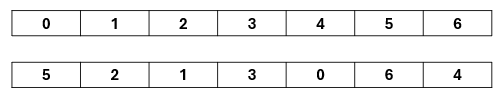
\includegraphics[width=0.8\textwidth]{
        papers/varalg/images/teil3/02GeneticStringCities.png
        }
	\caption{Beispiel von Städten in einem genetischen String dargestellt}
	\label{fig:cities_genetic_string}
\end{figure}

%
% teil3.tex -- Beispiel-File für Teil 3
%
% (c) 2020 Prof Dr Andreas Müller, Hochschule Rapperswil
%
% !TEX root = ../../buch.tex
% !TEX encoding = UTF-8
%
\subsection{Evaluation
\label{buch:paper:varalg:subsection:evaluation}}
\rhead{Evaluation}
Dieser Schritt befasst sich mit der auswertung der einzelnen 
Kombinationen.

In der Informatik wird die Liste genommen und die einzelnen 
Zusammenstellung wird berechnet.

Dafür wird die gleiche Formel \ref{eq:bruteforce_min_formula}, 
verwendet, die auch im Bruteforce-Methode Anwendung findet.

\begin{figure}
	\centering
	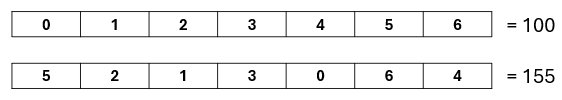
\includegraphics[width=0.8\textwidth]{
        papers/varalg/images/teil3/03GeneticStringCitiesResults.png
        }
	\caption{Beispiel eines genetischen Strings mit Ergebnissen}
	\label{fig:cities_genetic_string_results}
\end{figure}


%
% teil3.tex -- Beispiel-File für Teil 3
%
% (c) 2020 Prof Dr Andreas Müller, Hochschule Rapperswil
%
% !TEX root = ../../buch.tex
% !TEX encoding = UTF-8
%
\subsection{Selektion
\label{buch:paper:varalg:subsection:selection}}
\rhead{Selektion}
In diesem Schritt werden Elternpaare ausgewählt, aus denen neue 
Nachkommen erzeugt werden. Die Selektion erfolgt so, dass in der 
Regel nur die Fittesten die Chance erhalten, neue Kinder zu erzeugen. 
Ein wichtiger Punkt ist, dass, obwohl die Fittesten bevorzugt werden, 
auch die weniger Fitten die Möglichkeit haben, Nachkommen zu erzeugen. 
Dadurch wird sichergestellt, dass die Population nicht zu schnell 
konvergiert\footnote{
    Konvergenz bedeutet, dass die Population von Lösungen immer ähnlicher wird
    }
und in einem lokalen Minimum stecken bleibt. Durch die weniger Geeigneten 
wird die Vielfalt der Population erhalten und somit die Chance erhöht, 
dass die Population nicht in einem lokalen Minimum steckenbleibt. Die Abbildung
\ref{fig:selection_of_parents} stellt dies bildlich dar.
\begin{figure}
    \centering
    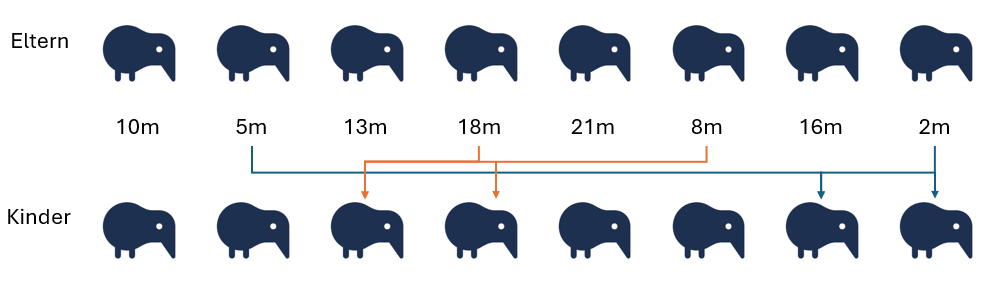
\includegraphics[width=0.8\textwidth]{
        papers/varalg/images/teil3/04OffspringProbability.png
    }
    \caption{
        Mögliche ausgewählte Eltern für Nachkommen, wobei die blaue Linie 
        eine höhere Wahrscheinlichkeit hat als die rote Linie}
    \label{fig:selection_of_parents}
\end{figure}
Für die Selektion gibt es verschiedene Möglichkeiten.
\begin{enumerate}
    \item \textbf{Roulette-Rad-Selektion:} Individuen werden zufällig und
    proportional zu ihrer Fitness ausgewählt. Die Wahrscheinlichkeit wird 
    anhand ihrer Fitness definiert. Kürzere Strecken haben eine höhere Chance, 
    ausgewählt zu werden. Die Wahrscheinlichkeit lässt sich mit der Formel
    \begin{align}
        \[
            P_i
            =
            \frac{f_i}{\sum_{j=1}^{N} f_j}
        \]
        \label{buch:paper:varalg:subsection:selection:probability_fittest}
    \end{align}
    berechnen. \(f_i\) ist die Funktion, welche die Fitness des Individuums berechnet.
    Geteilt durch die Totale Fitness. \(P_i\) ist die Wahrscheinlichkeit für das Individuum
    \item \textbf{Rangselektion:} Individuen werden nach ihrer Fitness sortiert und basierend
    auf ihrem Rang ausgewählt. Die Wahrscheinlichkeit wird anhand des Rangs definiert. Die 
    Formel 
    \begin{align}
        \[
            P_i
            =
            \frac{r_i}{\sum_{j=1}^{N} r_j}
        \]
        \label{buch:paper:varalg:subsection:selection:probability_rating}
    \end{align}
    ist die gleiche wie oben, verwendet jedoch die Funktion \(r_i\), welche den 
    Rang des Individuums berechnet.
    \item \textbf{Turnierselektion:} Eine Gruppe von Individuen wird zufällig ausgewählt
    und das fitteste Individuum dieser Gruppe wird als Elternteil gewählt.
\end{enumerate}
Es gibt auch die Möglichkeit, ein eigenes Selektionssystem zu entwickeln, 
das ein Ausscheidungsverfahren beinhaltet, aus dem schliesslich ein 
Elternpaar hervorgeht. Das System folgt einem logischen Ablauf, wobei 
die Wahrscheinlichkeit mathematisch berechnet wird.

\subsection{Selektion auf das TSP angepasst
\label{buch:paper:varalg:subsection:selection_tsp}}
\rhead{Selektion TSP}
Für das Traveling Salesman Problem muss die Fitness nach der kürzeste Strecke,
definiert sein. Dass bedeutet, dass die Wahrscheinlichkeit für die Selektion
so umgestellt werden, dass je kürzer die Strecke, desto höher die Wahrscheinlichkeit
ist. Die Formel \ref{buch:paper:varalg:subsection:selection:probability_fittest} wird 
dafür angepasst und neu zu
\begin{align}
    \[
        P_i
        =
        \frac{\frac{1}{f_i}}{\sum_{j=1}^{N} \frac{1}{f_j}}
    \]
    \label{buch:paper:varalg:subsection:selection:probability_fittest_tsp}
\end{align}
, dabei wird die Fitness mit \(\frac{1}{f_i}\) umgekehrte.

%
% teil3.tex -- Beispiel-File für Teil 3
%
% (c) 2020 Prof Dr Andreas Müller, Hochschule Rapperswil
%
% !TEX root = ../../buch.tex
% !TEX encoding = UTF-8
%
\subsection{Kreuzung
\label{buch:paper:varalg:subsection:crossover}}
\index{Kreuzung}%
In diesem Schritt des Algorithmus werden aus den gewählten Elternpaaren 
neue Nachkommen erzeugt. Dies wird erreicht, indem Teile des genetischen 
Strings miteinander ausgetauscht werden, 
wie in der Abbildung \ref{fig:one_point_crossover} veranschaulicht.
Durch diesen Mechanismus wird die Variation aufrechterhalten. Wichtig ist es,
dass aus zwei Eltern immer genau zwei Nachkommen erzeugt werden. Würde
die Population wachsen, würde der Aufwand zwischen den Generationen
wachsen, was den Zweck des Algorithmus verfehlt. Daher muss die Grösse der
Population immer konstant bleiben.
\begin{figure}
	\centering
	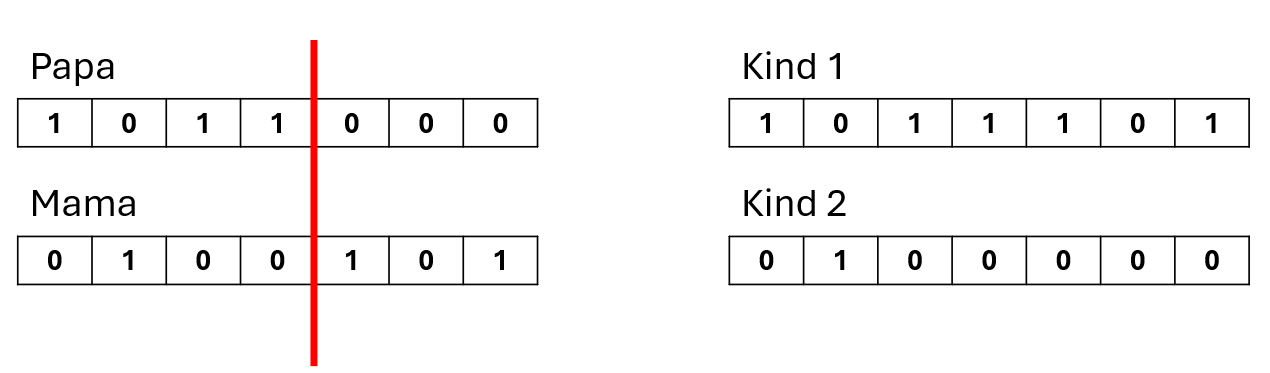
\includegraphics[width=0.8\textwidth]{
		papers/varalg/images/teil3/05GeneticStringCross.png
	}
	\caption{Ein einfaches Beispiel für eine Einpunkt-Kreuzung}
	\label{fig:one_point_crossover}
\end{figure}
Für die Kreuzung gibt es unterschiedliche Methoden, die gebräuchlichsten sind
die folgenden:
\begin{itemize}
	\item \textbf{Einpunkt-Kreuzung:} Ein zufälliger Punkt \( k \) \((1 \leq k < n)\)
\index{Einpunkt-Kreuzung}%
	wird auf den Elternchromosomen ausgewählt. Der Teil vor diesem Punkt stammt
	von einem Elternteil, die Gene ab diesem Punkt kommen vom anderen Elternteil. 
	Für die Erzeugung der Nachkommen wird mit den Formeln
	\begin{align*}
		O_1 = (P_1[1], P_1[2], \ldots, P_1[k], P_2[k+1], \ldots, P_2[n])\\
		O_2 = (P_2[1], P_2[2], \ldots, P_2[k], P_1[k+1], \ldots, P_1[n])
	\end{align*}
	gearbeitet. Die Abbildung \ref{fig:one_point_crossover} stellt diese Kreuzung bildlich dar.
	\item \textbf{Zweipunkt-Kreuzung:} Zwei zufällige Punkte \( k_1 \) und \( k_2 \)
\index{Zweipunkt-Kreuzung}%
	\((1 \leq k_1 < k_2 < n)\) werden ausgewählt und
	der Genabschnitt zwischen diesen Punkten wird zwischen den Eltern 
	getauscht. Die Nachkommen werden durch die Formeln
	\begin{align*}
		O_1 = (P_1[1], \ldots, P_1[k_1], P_2[k_1+1], \ldots, P_2[k_2], P_1[k_2+1], \ldots, P_1[n])\\
		O_2 = (P_2[1], \ldots, P_2[k_1], P_1[k_1+1], \ldots, P_1[k_2], P_2[k_2+1], \ldots, P_2[n])
	\end{align*}
	erzeugt.
	\item \textbf{Uniforme Kreuzung:} Jedes Gen wird mit einer bestimmten
\index{Kreuzung, uniform}%
\index{uniforme Kreuzung}%
	Wahrscheinlichkeit vom ersten oder zweiten Elternteil übernommen, was zu
	einer zufälligeren Kombination führt. Für jedes Gen \( i \) \((1 \leq i \leq n)\)
	wird eine zufällige Zahl \( r_i \) im Intervall [0, 1] gewählt. Wenn
	\( r_i \) kleiner als die vordefinierte Wahrscheinlichkeit \( p \) ist,
	dann wird das Gen von \( P_1 \) übernommen, ansonsten von \( P_2 \). Es
	wird über jede Position mit der Formel 
	\begin{align*}
		O_1[i] &=
		\begin{cases} 
			P_1[i] & \text{wenn } r_i < p       \\
			P_2[i] & \text{wenn } r_i \geq p 
		\end{cases}
		\\
		O_2[i] &=
		\begin{cases} 
			P_2[i] & \text{wenn } r_i < p       \\
			P_1[i] & \text{wenn } r_i \geq p 
		\end{cases}
	\end{align*}
	iteriert.
% 	Wissenstand der Leser ist vorausgesetzt
%	\footnote{
%		Iterieren wird typischerweise in der Informatik verwendet und 
%		bedeutet, dass über eine Menge der Reihe nach durchgegangen wird. 
%		Bei der Iteration über einen String wird jede Position des Strings 
%		angeschaut und je nach Aufgabe etwas mit diesem Zeichen gemacht.
%		}.
\end{itemize}

\subsubsection{Kreuzung auf das TSP angepasst
\label{buch:paper:varalg:subsection:crossover_tsp}}
Für das Travelling-Salesman-Problem muss der Algorithmus angepasst werden.
Würde das System wie in der Abbildung \ref{fig:one_point_crossover} 
übernommen werden, würde das Resultat unkorrekte Teile enthalten, was zu einem 
String wie in der Abbildung \ref{fig:one_point_crossover_cities} führt.
\begin{figure}
	\centering
	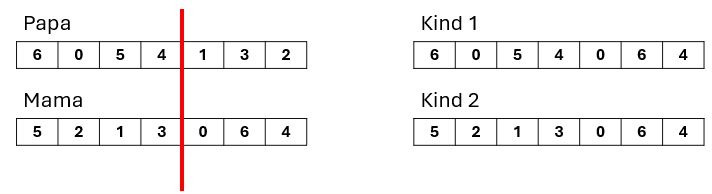
\includegraphics[width=0.8\textwidth]{
		papers/varalg/images/teil3/07GeneticStringCitiesCrossoverStandard.png
	}
	\caption{Beispiel einer Einpunkt-Kreuzung mit Städten ohne Anpassungen.}
	\label{fig:one_point_crossover_cities}
\end{figure}
Daher wird der Algorithmus so angepasst, dass keine Städte verschwinden
oder doppelte auftreten. Die einfachste Methode ist es, den Teil, der ersetzt wird,
zu entfernen und danach die fehlenden Teile nach der Reihenfolge des anderen
Elternteils zu ergänzen, bis der String wieder vollständig ist. Ein visuelles Beispiel
finden Sie in der Abbildung \ref{fig:crossover_order_cities}.
\begin{figure}
	\centering
	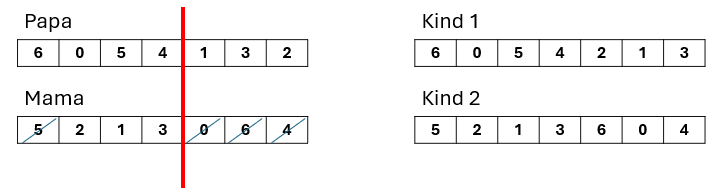
\includegraphics[width=0.8\textwidth]{
		papers/varalg/images/teil3/08GeneticStringCitiesCrossoverSimple.png
	}
	\caption{
		Beispiel einer Einpunkt-Kreuzung, welche angepasst an das TSP ist. Der ersetzende Teil wurde entfernt und
		nach der Reihenfolge des anderen Elternteils ergänzt.
	}
	\label{fig:crossover_order_cities}
\end{figure}

%
% teil3.tex -- Beispiel-File für Teil 3
%
% (c) 2020 Prof Dr Andreas Müller, Hochschule Rapperswil
%
% !TEX root = ../../buch.tex
% !TEX encoding = UTF-8
%
\subsection{Mutation
\label{buch:paper:varalg:subsection:mutation}}
\rhead{Mutation}
Dieser Schritt sorgt dafür, dass zufällige Änderungen in 
den Genen stattfinden. Dadurch entstehen neue Gene, was den 
gesamten Lösungsraum vergrössert. Zusätzlich soll es verhindern,
dass nach einer Anzahl von Generationen immer wieder die
gleichen Genmuster entstehen, wodurch verhindert werden soll, dass 
der Algorithmus in einem lokalen Extrempunkt stecken bleibt. 
Die Mutation findet auch nicht bei jedem Kind
statt, sondern wie in der Natur werden diese per Zufall
ausgelöst. Die Mutation läuft so ab, dass über den String
iteriert wird und jedes Mal wird eine Zufallszahl erzeugt. Wird 
die Bedingung im Zusammenhang mit der erzeugten Zahl erfüllt, dann wird 
die Stelle invertiert, wie in der
Abbildung \ref{fig:mutation_genetic_string} dargestellt. Dieser Schritt 
lässt Variationen entstehen, die bei der Kreuzung nicht entstanden wären. 
\begin{figure}
	\centering
	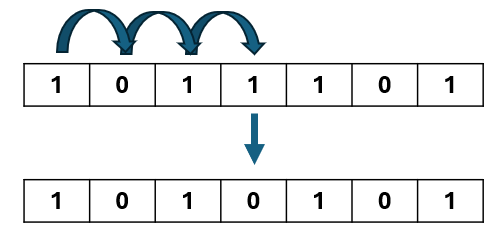
\includegraphics[width=0.8\textwidth]{
        papers/varalg/images/teil3/09GeneticStringMutation.png
        }
	\caption{
	Beispiel einer Mutation mit einem genetischen String aus 0 und 1. Die
	Mutation wird zufällig ausgelöst und invertiert die Stelle.
	}
	\label{fig:mutation_genetic_string}
\end{figure}

\subsection{Mutation auf das TSP angepasst
\label{buch:paper:varalg:subsection:mutation_tsp}}
\rhead{Mutation TSP}
Für das Travelling Salesman Problem wird die Mutation so angepasst,
dass, wenn eine Mutation stattfindet, zwei zufällige Stellen ausgewählt
werden und diese Städte vertauscht werden, 
wie in der Abbildung \ref{fig:mutation_genetic_string_cities}.
\begin{figure}
	\centering
	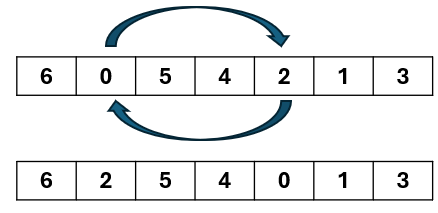
\includegraphics[width=0.8\textwidth]{
        papers/varalg/images/teil3/09GeneticStringCitiesMutation.png
        }
	\caption{Beispiel einer Mutation mit Städten}
	\label{fig:mutation_genetic_string_cities}
\end{figure}

%
% teil3.tex -- Beispiel-File für Teil 3
%
% (c) 2020 Prof Dr Andreas Müller, Hochschule Rapperswil
%
% !TEX root = ../../buch.tex
% !TEX encoding = UTF-8
%
\subsection{Ersetzen
\label{varalgbuch:paper:varalg:subsection:replacement}}
\rhead{Ersetzen}
Der Ersetzungsschritt macht, was er aussagt. Meistens wird die ganze 
Population durch die neue ersetzt, sodass mit einer neuen Generation gearbeitet wird.
Es gibt aber auch die Möglichkeit, einen Teil zu erhalten. Dazu setzt man eine 
Grenze fest und dieser wird in die neue Population übertragen. Man erhofft sich so, 
dass aus den besten Lösungen beider Generationen noch bessere entstehen.
Wichtig ist, dass die Gesamtgrösse der Population gleich bleibt.

\subsection{Ersetzen auf das TSP angepasst
\label{buch:paper:varalg:subsection:replacement_tsp}}
\rhead{Ersetzen TSP}
Dieser Schritt kann auf das TSP angewendet werden, ohne weitere
Anpassungen vorzunehmen.

%
% teil3.tex -- Beispiel-File für Teil 3
%
% (c) 2020 Prof Dr Andreas Müller, Hochschule Rapperswil
%
% !TEX root = ../../buch.tex
% !TEX encoding = UTF-8
%
\subsection{Abbruchkriterium
\label{buch:paper:varalg:subsection:termination}}
\rhead{Abbruchkriteriums}
Wie auch im maschinellen Lernen ist es wichtig zu bestimmen, unter 
welchen Bedingungen der Vorgang beendet werden soll. Beim 
genetischen Algorithmus wird in der Regel eine maximale Anzahl an 
Generationen definiert. Eine weitere Möglichkeit besteht darin, 
die Berechnungen zu beenden, sobald ein gewisser Fitnesswert erreicht 
wird und die Lösung als ausreichend angesehen werden kann.

\subsection{Abbruchkriterium auf das TSP angepasst
\label{buch:paper:varalg:subsection:termination_tsp}}
\rhead{Abbruchkriteriums TSP}
Für das Travelling Salesman Problem sind beide Abbruchkriterien im 
Abschnitt \ref{buch:paper:varalg:subsection:termination} anwendbar.

